% Created 2023-06-06 Tue 00:05
% Intended LaTeX compiler: pdflatex
\documentclass[11pt]{article}
\usepackage[utf8]{inputenc}
\usepackage[T1]{fontenc}
\usepackage{graphicx}
\usepackage{longtable}
\usepackage{wrapfig}
\usepackage{rotating}
\usepackage[normalem]{ulem}
\usepackage{amsmath}
\usepackage{amssymb}
\usepackage{capt-of}
\usepackage{hyperref}
\author{Barak-Nadav Diker}
\date{\today}
\title{}
\hypersetup{
 pdfauthor={Barak-Nadav Diker},
 pdftitle={},
 pdfkeywords={},
 pdfsubject={},
 pdfcreator={Emacs 28.2.50 (Org mode 9.6.1)}, 
 pdflang={English}}
\begin{document}



\section*{Definition}
\label{sec:orgfb98bf2}
Pagerank is an algorithm used by google search to rank web pages
in their search engine

In Simpler words : PageRank is a way of measuring the importance of a website

\section*{Notable quote by google}
\label{sec:orgb6d0d5c}
PageRank works by counting the number and quality of links to a page to determine a rough estimate of how important the website is. The underlying assumption is that more important websites are likely to receive more links from other websites.
\section*{Nice to know}
\label{sec:orge745c3b}
\textbf{PageRank and all associated patent are expired !!}



\section*{So What's the formula ?}
\label{sec:orgfbc1dac}
The Naive algorithm is the following formula

\[ PR(u) = \sum_{v \in B_u}\frac{PR(v)}{L(v)} \]

Where \(L \colon V \to \mathbb{N}\) is number of outbounds links
and \(PR \colon V \to [0,1]\) is the PageRank of a vertex
and the initial probability is \(\forall v \in V , PR(v)=\frac{1}{|V|}\)



\section*{Simple Example}
\label{sec:org61f9a39}

Note the following graph

\begin{verbatim}
    PR(A) = 0.25
    PR(B) = 0.25
    PR(C) = 0.25
    PR(D) = 0.25
\end{verbatim}

\begin{center}
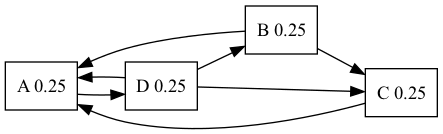
\includegraphics[width=.9\linewidth]{simple_example1.png}
\end{center}



\subsection*{After first iteration}
\label{sec:org04aaf51}
We'll Calculate explicitly for PR(A)

\[ PR(A)= \frac{PR(B)}{L(B)} + \frac{PR(C)}{L(C)} + \frac{PR(D)}{L(D)} \]
\[ PR(A)= \frac{0.25}{2} +  \frac{0.25}{1} + \frac{0.25}{3}\]



\begin{center}
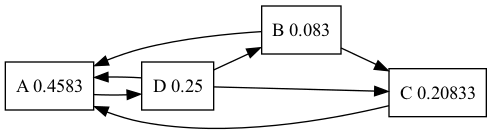
\includegraphics[width=.9\linewidth]{another_example1.png}
\end{center}

\section*{Is there a problem ?}
\label{sec:orge0099ff}

\begin{itemize}
\item If a page has no links to other pages, it becomes a sink and therefore terminates the random surfing process!
\end{itemize}
Sound vague .. Why is it a problem ?





\section*{intuition}
\label{sec:org8940000}
In Each iteration every note ``passes'' all his probability to it's outbound neighbours

but if one of the notes doesn't have outbound edges he'll receive probability but the note won't export his probablity

So the sum of the probability of all nodes \(\sum_{v \in V}PR(v) = 1-PR(v_i) < 1\) where \(v_i\) is the probability of sink in the previous iteration



\section*{Example}
\label{sec:orgb5d7f76}
Example with sink
\begin{center}
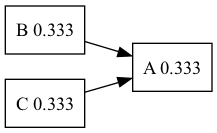
\includegraphics[width=.9\linewidth]{sink_problem1.png}
\end{center}


\subsection*{in the first iteration}
\label{sec:org8bc586f}
Note that node B and node C passes all it's probability to node A
And node A passes 0.333 to nobody !
\begin{center}
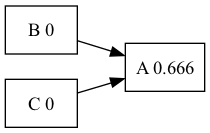
\includegraphics[width=.9\linewidth]{sink_problem2.png}
\end{center}

\section*{Another Problem}
\label{sec:org274a42f}
Another Problem might occur if we have inside our graph infinite cycle

like in the following graph

All the PageRank would go into node a and node b

\begin{center}
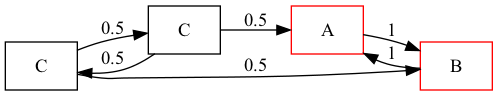
\includegraphics[width=.9\linewidth]{inifinite_cycle.png}
\end{center}


\section*{Damping Factor}
\label{sec:org07c9da5}
solution : if we'll reach a sink we'll jump to a random note (Uniformly)
by the formula
\[ PR(p_{i})= \frac{1-d}{N} + d \sum_{p_{j} \in B_{p_i}} \frac{PR(p_j)}{L(p_j)} \]
Where d is usually 0.85 i.e \(d=0.85\) and \(B_{p_i}\) is the set containing all pages linking to page u
and \(L(p_j)\) is the number of links from \(p_j\)

Why will it work ?? how ??





\section*{A more general notation}
\label{sec:orga19cf7a}
note that we can write the formula more compactly like so

\begin{equation}
\mathbf{R} =
\begin{bmatrix}
PR(p_1) \\
PR(p_2) \\
\vdots \\
PR(p_N)
\end{bmatrix}
\end{equation}

where '''R''' is the solution of the equation
\subsection*{The full equation}
\label{sec:org5756a7d}


\begin{equation}
\mathbf{R} =
\begin{bmatrix}
{(1-d)/ N} \\
{(1-d) / N} \\
\vdots \\
{(1-d) / N}
\end{bmatrix}
\\ + d
\begin{bmatrix}
\ell(p_1,p_1) & \ell(p_1,p_2) & \cdots & \ell(p_1,p_N) \\
\ell(p_2,p_1) & \ddots &  & \vdots \\
\vdots & & \ell(p_i,p_j) & \\
\ell(p_N,p_1) & \cdots & & \ell(p_N,p_N)
\end{bmatrix}
\mathbf{R}
\end{equation}
\subsection*{Continue}
\label{sec:orgd5ecc5b}
where the adjacency function \(\ell( p_i , p_j )\) is the ratio between number of links outbound from page j to page i to the total number of outbound links of page j.
\begin{equation} \sum_{i = 1}^N \ell(p_i,p_j) = 1 \end{equation}



\subsection*{The Algorithm}
\label{sec:orgafef686}
If the matrix \({\mathcal {M}}\) is a transition probability, i.e., column-stochastic and \(\mathbf{R}\) is a probability distribution
\begin{itemize}
\item \(\|\mathbf{R}\|=1, \mathbf{E}\mathbf{R}=\mathbf{1}\) where \(\mathbf{E}\) is matrix of all ones
\end{itemize}

\[ \mathbf{R} = \left( d \mathcal{M} + \frac{1-d}{N} \mathbf{E} \right)\mathbf{R} =: \widehat{ \mathcal{M}} \mathbf{R} \]

\subsection*{Continue}
\label{sec:orge8d415a}
Hence PageRank  \(\mathbf{R}\) is the principal eigenvector of \(\widehat{\mathcal{M}}\). A fast and easy way to compute this is using the power method: starting with an arbitrary vector  x(0), the operator \(\widehat{\mathcal{M}}\) is applied in succession, i.e.,

\[ x(t+1) = \widehat{\mathcal{M}} x(t), \]

until

\[ |x(t+1) - x(t)| <  \epsilon \]



\subsection*{Simple Implementation}
\label{sec:orgf34781d}
\begin{verbatim}
import numpy as np
def pagerank(M, num_iterations: int = 100, d: float = 0.85):
    N = M.shape[1]
    v = np.ones(N) / N
    M_hat = (d * M + (1 - d) / N)
    for i in range(num_iterations):
        v = M_hat @ v
    return v
M = np.array([[0  , 0, 0 , 0, 1],
              [0.5, 0, 0 , 0, 0],
              [0.5, 0, 0 , 0, 0],
              [0  , 1,0.5, 0, 0],
              [0  , 0,0.5, 1, 0]])
v = pagerank(M, 100, 0.85)
print(v)
\end{verbatim}

\section*{Markov Chain}
\label{sec:org1f68fba}
Let's be more formal !
Given a Graph and initial probability vector \(\pi _0 \in \mathbb{R}^n\)  where n is the number of vertaces ,
Define the Matrix P to be \([P]_{ij}\) the probability of going from node i to node j
Define \(\forall j \in [0,n]\bigcap \mathbb{N} , \vec \pi _{n+1} (j) = \vec \pi _n \cdot \vec P_{i,j}\)
\subsection*{More definition}
\label{sec:org8770bd6}
we want to find a unique stationary
distribution \(\lim\limits_{n\to \infty} \pi _n = \pi\) and Rank the Web Pages via that unique stationary distribution !

\subsection*{Example}
\label{sec:org2123d79}
Observe the following graph
\[ \pi _{n+1}(0) = \pi _n \cdot P(0,0) + \pi _n \cdot P(1,0) +\pi _n \cdot P(2,0) \\ +\pi _n \cdot P(3,0) + \pi _n \cdot P(4,0) \]

\begin{center}
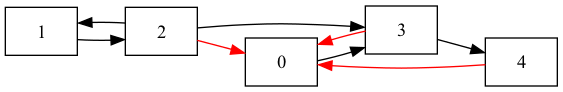
\includegraphics[width=.9\linewidth]{markov_simple_calc.png}
\end{center}



\section*{Serious questions}
\label{sec:org7d9549c}
\begin{itemize}
\item Is there unique stationary distribution ?
Certainly it would be hard to evaluate web pages if there are couple of stationary distribution
\item Does every initial distribution converges to the stationary one ?
if so how to pick initial distribution ?
\end{itemize}
serious question \ldots{} maybe mathematics could help us ??

\section*{First question}
\label{sec:orgc561b6b}
Can you define a Markov chain with multiple stationary distributions ?

Think of markov chain with only 2 states \ldots{}

\subsection*{The Answer}
\label{sec:org1fc2dc5}
This graph has multiple stationary solutions

\begin{center}
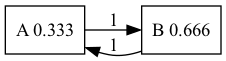
\includegraphics[width=.9\linewidth]{multi_stationary_distribution1.png}
\end{center}

\begin{center}
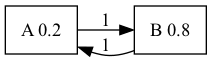
\includegraphics[width=.9\linewidth]{multi_stationary_distribution2.png}
\end{center}



\subsection*{Another Example}
\label{sec:org70c2201}
Can we Think of another example ??
Graph that isn't strongly connect .i.e exists 2 nodes such that we cannot create a path from the former to the latter

interestingly , That is one of the definition of ``Reducible Markov Chain''

Let's see the example !



\subsection*{Visulaize}
\label{sec:orgb05e430}
There isn't a path between node 0 into node 1 i.e this graph isn't reducible
So again the stationary solution isn't unique !!

\begin{center}
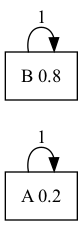
\includegraphics[width=.9\linewidth]{not_strongly_connected.png}
\end{center}

\subsection*{Conclusion}
\label{sec:org1202b03}
The first graph was periodic markov chain
and the second graph was reducible markov chain

apparently The answer is yes to the 2 previous question if
the graph is aperiodic and irreducible markov chain


\subsection*{Theorem}
\label{sec:org3e2336e}
if graph is Irreducible markov chain i.e all state are reachable \(\rightarrow\) there is unique stationary distribution

Note , The first example has a unique stationary distribution (0.5 0.5)
All other solutions aren't stationary for example (0.3 0.7) would oscilate between them


\section*{The second question}
\label{sec:org61c1f9e}
Does every initial distribution converge to the stationary one ?

Clarification ! for all initial distribution we want to converge to \textbf{the} stationary one

Give me an irreducible markov chain where the stationary distribution does not converge
we have already counter-example , so what else we need to assume on the graph ?


\section*{Periodic Markov Chain}
\label{sec:org7151029}
\begin{itemize}
\item Must be an irreducible markov chain
\item User visits states in regular interval (period) > 1
(There is a better definition)
\end{itemize}
So Given an Periodic Markov Chain There is no guarantee of convergence to stationary distribution

If no such period exists > 1 , then we said that the graph is Aperiodic Markov Chain

\section*{Ergodic Theorem}
\label{sec:org02593a4}
For Irreducible and aperiodic markov chains:
\begin{enumerate}
\item A unique stationary distribution \(\pi\) exists
\item All initial distribution \(\pi _0\) converges to that unique stationary distribution \(\pi\)
\end{enumerate}

\section*{How fast does the solution converges ?}
\label{sec:orgcf2b619}
Because of the large eigengap of the modified adjacency matrix above, the values of the PageRank eigenvector can be approximated to within a high degree of accuracy within only a ``few'' iterations.

\href{https://en.wikipedia.org/wiki/Eigenvalue\_perturbation}{Davis–Kahan theorem}

But What is ``few'' ?

log(n)

\section*{The End}
\label{sec:orga1b9d75}
End !

\section*{To delete}
\label{sec:org22751a2}
Column 1
Column 2


\section*{To delete}
\label{sec:org0895524}
Box 1
Box 2
Box 3

\section*{Some Notable code}
\label{sec:org0466460}

\begin{verbatim}
int main()
{
  cout << "Hello" << endl;
}
\end{verbatim}
\section*{Slide 1}
\label{sec:org850f45b}
\begin{itemize}
\item List item 1
\end{itemize}

\begin{center}
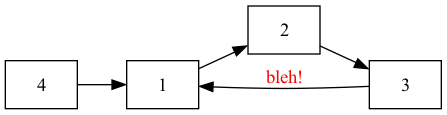
\includegraphics[width=.9\linewidth]{test1.png}
\end{center}

\begin{itemize}
\item List item 2
\end{itemize}

\begin{center}
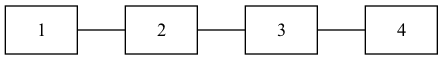
\includegraphics[width=.9\linewidth]{test2.png}
\end{center}

\section*{Nice Code Animation}
\label{sec:org47059b4}
\begin{verbatim}
  let index = 1
\end{verbatim}


\subsection*{Added value}
\label{sec:orgc05d471}
\begin{verbatim}
  let index = 1
  let value = 2
\end{verbatim}

\section*{some equation}
\label{sec:org9a9442a}
\[ \sin(x) = \frac{1}{n} \]
\end{document}